\documentclass[]{article}
\usepackage[left=1in,top=1in,right=1in,bottom=1in]{geometry}


%%%% more monte %%%%
\usepackage{wrapfig}
% thispagestyle{empty}
% https://stackoverflow.com/questions/2166557/how-to-hide-the-page-number-in-latex-on-first-page-of-a-chapter
\usepackage{color}
% \usepackage[table]{xcolor} % are they using color?

% \definecolor{WSU.crimson}{HTML}{981e32}
% \definecolor{WSU.gray}{HTML}{5e6a71}

% \definecolor{shadecolor}{RGB}{248,248,248}
\definecolor{WSU.crimson}{RGB}{152,30,50} % use http://colors.mshaffer.com to convert from 981e32
\definecolor{WSU.gray}{RGB}{94,106,113}

%%%%%%%%%%%%%%%%%%%%%%%%%%%%

\newcommand*{\authorfont}{\fontfamily{phv}\selectfont}
\usepackage{lmodern}


  \usepackage[T1]{fontenc}
  \usepackage[utf8]{inputenc}




\usepackage{abstract}
\renewcommand{\abstractname}{}    % clear the title
\renewcommand{\absnamepos}{empty} % originally center

\renewenvironment{abstract}
 {{%
    \setlength{\leftmargin}{0mm}
    \setlength{\rightmargin}{\leftmargin}%
  }%
  \relax}
 {\endlist}

\makeatletter
\def\@maketitle{%
  \pagestyle{empty}
  \newpage
%  \null
%  \vskip 2em%
%  \begin{center}%
  \let \footnote \thanks
    {\fontsize{18}{20}\selectfont\raggedright  \setlength{\parindent}{0pt} \@title \par}%
}
%\fi
\makeatother









\title{\textbf{\textcolor{WSU.crimson}{Value proposition for the
Data-analytics Program}} \newline \textbf{\textcolor{WSU.gray}{What can
we learn from market demand?}}  }
 

%  

% \author{ \Large true \hfill \normalsize \emph{} }
\author{\Large Monte J.
Shaffer\vspace{0.05in} \newline\normalsize\emph{Ph.D.~(Marketing, WSU
'11), M.S. (Statistics WSU '11), MBA (Marketing, BYU '06)}  }


\date{April 12, 2021}
\setcounter{secnumdepth}{3}

\usepackage{titlesec}
% See the link above: KOMA classes are not compatible with titlesec any more. Sorry.
% https://github.com/jbezos/titlesec/issues/11
\titleformat*{\section}{\bfseries}
\titleformat*{\subsection}{\bfseries\itshape}
\titleformat*{\subsubsection}{\itshape}
\titleformat*{\paragraph}{\itshape}
\titleformat*{\subparagraph}{\itshape}

% https://code.usgs.gov/usgs/norock/irvine_k/ip-092225/


%\titleformat*{\section}{\normalsize\bfseries}
%\titleformat*{\subsection}{\normalsize\itshape}
%\titleformat*{\subsubsection}{\normalsize\itshape}
%\titleformat*{\paragraph}{\normalsize\itshape}
%\titleformat*{\subparagraph}{\normalsize\itshape}

% https://tex.stackexchange.com/questions/233866/one-column-multicol-environment#233904
\usepackage{environ}
\NewEnviron{auxmulticols}[1]{%
  \ifnum#1<2\relax% Fewer than 2 columns
    %\vspace{-\baselineskip}% Possible vertical correction
    \BODY
  \else% More than 1 column
    \begin{multicols}{#1}
      \BODY
    \end{multicols}%
  \fi
}





\usepackage{natbib}
\setcitestyle{aysep={}} %% no year, comma just year
% \usepackage[numbers]{natbib}
\bibliographystyle{./../../latex-setup/biblio/ormsv080.bst}



\usepackage[strings]{underscore} % protect underscores in most circumstances




\newtheorem{hypothesis}{Hypothesis}
\usepackage{setspace}


%%%%%%%%%%%%%%%%%%%%%%%%%%%%%%%%%%%%%%%%%%%%%%%%%%%%%
%%% MONTE ADDS %%%

\usepackage{fancyhdr} % fancy header 
\usepackage{lastpage} % last page 

\usepackage{multicol}


\usepackage{etoolbox}
\AtBeginEnvironment{quote}{\singlespacing\small}
% https://tex.stackexchange.com/questions/325695/how-to-style-blockquote


\usepackage{soul}			%% allows strike-through
\usepackage{url}			%% fixes underscores in urls
\usepackage{csquotes}		%% allows \textquote in references
\usepackage{rotating}		%% allows table and box rotation
\usepackage{caption}		%% customize caption information
\usepackage{booktabs}		%% enhance table/tabular environment
\usepackage{tabularx}		%% width attributes updates tabular
\usepackage{enumerate}		%% special item environment
\usepackage{enumitem}		%% special item environment

\usepackage{lineno}		%% allows linenumbers for editing using \linenumbers
\usepackage{hanging}


\usepackage{mathtools}  	%% also loads amsmath
\usepackage{bm}		%% bold-math
\usepackage{scalerel}	%% scale one element (make one beta bigger font)

\newcommand{\gFrac}[2]{ \genfrac{}{}{0pt}{1}{{#1}}{#2} }

\newcommand{\betaSH}[3]{  \gFrac{\text{\tiny #1}}{{\text{\tiny #2}}}\hat{\beta}_{\text{#3}}   }
\newcommand{\betaSB}[3]{              ^{\text{#1}} _{\text{#2}} \bm{\beta} _{\text{#3}}                   }  %% bold
\newcommand{\bigEQ}{  \scaleobj{1.5}{{\ }= } }
\newcommand{\bigP}[1]{  \scaleobj{1.5}{#1 } }





\usepackage{endnotes}  % he already does this ...
\renewcommand{\enotesize}{\normalsize}
% https://tex.stackexchange.com/questions/99984/endnotes-do-not-be-superscript-and-add-a-space
\renewcommand\makeenmark{\textsuperscript{[\theenmark]}} % in brackets %
% https://tex.stackexchange.com/questions/31574/how-to-control-the-indent-in-endnotes
\patchcmd{\enoteformat}{1.8em}{0pt}{}{}

\patchcmd{\theendnotes}
  {\makeatletter}
  {\makeatletter\renewcommand\makeenmark{\textbf{[\theenmark]} }}
  {}{}



% https://tex.stackexchange.com/questions/141906/configuring-footnote-position-and-spacing

\addtolength{\footnotesep}{5mm} % change to 1mm

\renewcommand{\thefootnote}{\textbf{\arabic{footnote}}}
\let\footnote=\endnote
%\renewcommand*{\theendnote}{\alph{endnote}}
%\renewcommand{\theendnote}{\textbf{\arabic{endnote}}}


\renewcommand*{\notesname}{ENDNOTES}

\makeatletter
\def\enoteheading{\section*{\notesname
  \@mkboth{\MakeUppercase{\notesname}}{\MakeUppercase{\notesname}}}%
  \mbox{}\par\vskip-2.3\baselineskip\noindent\rule{.5\textwidth}{0.4pt}\par\vskip\baselineskip}
\makeatother


\renewcommand*{\contentsname}{TABLE OF CONTENTS}

\renewcommand*{\refname}{REFERENCES}


%\usepackage{subfigure}
\usepackage{subcaption}

\captionsetup{labelfont=bf}  % Make Table / Figure bold

%%% you could add elements here ... monte says .... %%%
%\usepackage{mypackageForCapitalH}


%%%%%%%%%%%%%%%%%%%%%%%%%%%%%%%%%%%%%%%%%%%%%%%%%%%%%

% set default figure placement to htbp
\makeatletter
\def\fps@figure{htbp}
\makeatother


% move the hyperref stuff down here, after header-includes, to allow for - \usepackage{hyperref}

\makeatletter
\@ifpackageloaded{hyperref}{}{%
\ifxetex
  \PassOptionsToPackage{hyphens}{url}\usepackage[setpagesize=false, % page size defined by xetex
              unicode=false, % unicode breaks when used with xetex
              xetex]{hyperref}
\else
  \PassOptionsToPackage{hyphens}{url}\usepackage[draft,unicode=true]{hyperref}
\fi
}

\@ifpackageloaded{color}{
    \PassOptionsToPackage{usenames,dvipsnames}{color}
}{%
    \usepackage[usenames,dvipsnames]{color}
}
\makeatother
\hypersetup{breaklinks=true,
            bookmarks=true,
            pdfauthor={Monte J. Shaffer (Ph.D.~(Marketing, WSU '11),
M.S. (Statistics WSU '11), MBA (Marketing, BYU '06))},
             pdfkeywords = {data analytics; data science; market
demand},  
            pdftitle={Value proposition for the Data-analytics
Program: What can we learn from market demand?},
            colorlinks=true,
            citecolor=blue,
            urlcolor=blue,
            linkcolor=magenta,
            pdfborder={0 0 0}}
\urlstyle{same}  % don't use monospace font for urls

% Add an option for endnotes. -----

%
% add tightlist ----------
\providecommand{\tightlist}{%
\setlength{\itemsep}{0pt}\setlength{\parskip}{0pt}}

% add some other packages ----------

% \usepackage{multicol}
% This should regulate where figures float
% See: https://tex.stackexchange.com/questions/2275/keeping-tables-figures-close-to-where-they-are-mentioned
\usepackage[section]{placeins}



\pagestyle{fancy}   
\lhead{\textcolor{WSU.crimson}{\textbf{ Value proposition for the
Data-analytics Program }}}
\chead{}
\rhead{\textcolor{WSU.gray}{\textbf{  Page\ \thepage\ of\ \protect\pageref{LastPage} }}}
\lfoot{}
\cfoot{}
\rfoot{}


\begin{document}
	
% \pagenumbering{arabic}% resets `page` counter to 1 
%    

% \maketitle

{% \usefont{T1}{pnc}{m}{n}
\setlength{\parindent}{0pt}
\thispagestyle{plain}
{\fontsize{18}{20}\selectfont\raggedright 
\maketitle  % title \par  

}

{
   \vskip 13.5pt\relax \normalsize\fontsize{11}{12} 
   
\textbf{\authorfont Monte J.
Shaffer} \hskip 15pt \emph{\small Ph.D.~(Marketing, WSU '11), M.S.
(Statistics WSU '11), MBA (Marketing, BYU '06)}   

}

}








\begin{abstract}

    \hbox{\vrule height .2pt width 39.14pc}

    \vskip 8.5pt % \small 

\noindent University resources are limited. As such, any program
development should have a justifiable value proposition. In this
preliminary research, we explore the potential demand in the marketplace
for students earning undergraduate and advanced degrees in Data
Analytics. Preliminary analysis shows that \textbf{\tt{Data analytics}}
has greater job-market demand than \textbf{\tt{Data Science}} although
the latter has greater google-search demand. This data aligns with the
primary objectives of the data-analytics program at Washington State
University. \newline As such, we conclude that positioning our program
as \textbf{\tt{Data analytics}} is a justified value proposition.


\vskip 8.5pt \noindent \textbf{\underline{Keywords}:} data analytics;
data science; market demand \par

    




    
    \hbox{\vrule height .2pt width 39.14pc}
    \vskip 5pt 
    \hfill \textbf{\textcolor{WSU.gray}{ April 12, 2021 } }
    \vskip 5pt 
    
\end{abstract}


\vskip -8.5pt



 % removetitleabstract

\noindent  

\begin{figure}[!ht]
 \label{fig:one-graphic}
%% figures have hrule, tables have hline
    \begin{center}
        \scalebox{1.00}{    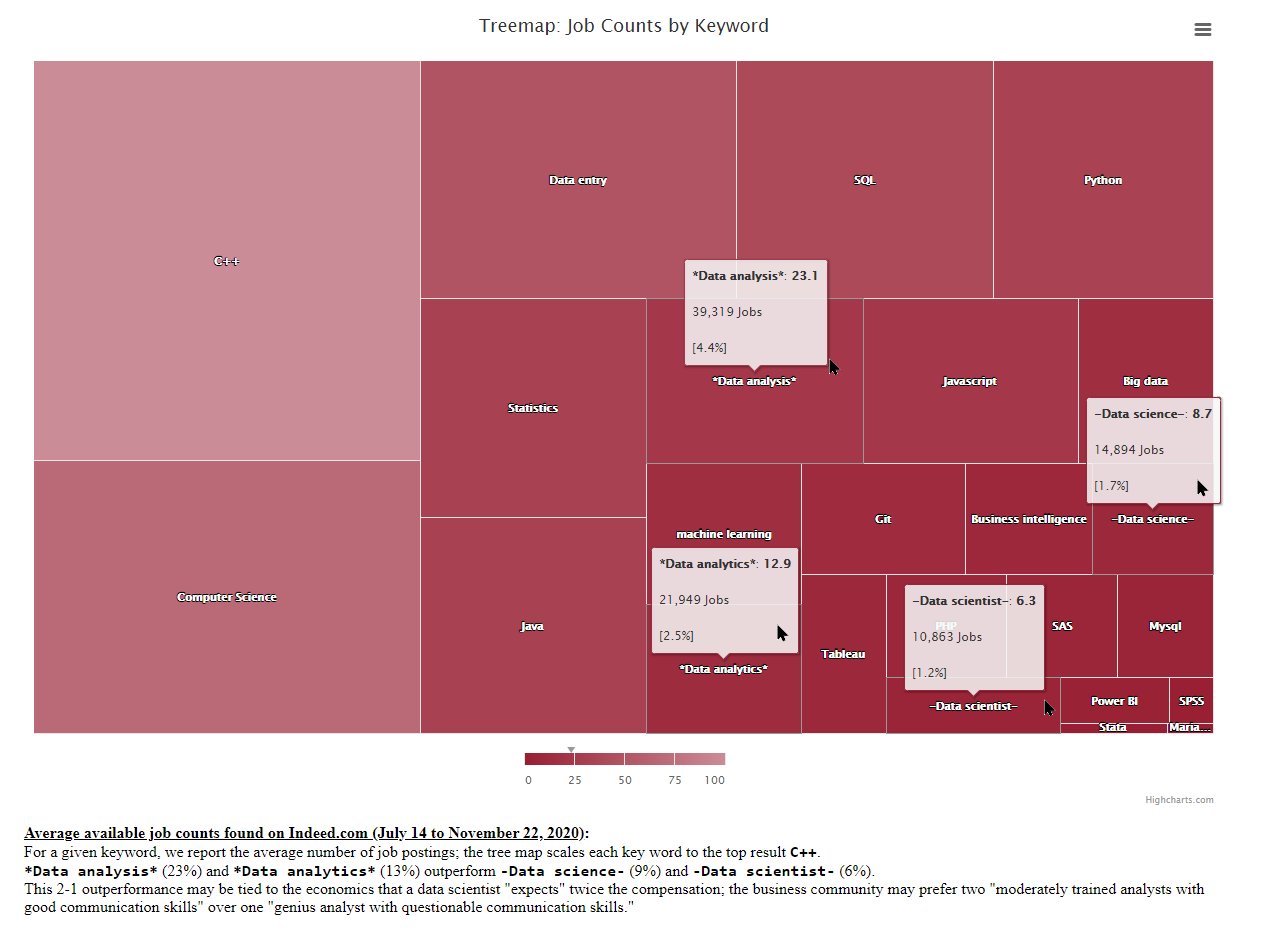
\includegraphics[trim = 0 50mm 0 5mm,clip,width=\textwidth]{figures/one.png} }
    \end{center}
    \hrule
      \vspace{2mm}
    \caption{ \textbf{Greater market demand for `data analytics' than for `data science':} \newline \footnotesize{ We report the average number of job posting for relevant keywords from the Indeed.com website (averaged with data collected from July 14 to November 22, 2020).  \newline \newline  All results are scaled as a proportion of the top result \textbf{\tt{C++}}. We observe that \textbf{\tt{Data analysis}} (23\%) and \textbf{\tt{Data analytics}} (13\%) outperform \textbf{\tt{Data science}} (9\%) and \textbf{\tt{Data scientist}} (6\%).  \newline \newline This 2-1 outperformance may be tied to the economics that a data scientist ``expects" twice the compensation; the business community may prefer two ``moderately trained analysts with good communication skills" over one ``genius analyst with questionable communication skills."  \newline \newline [High-resolution, interactive visualization: \url{https://bit.ly/39cA1Re}]}  }
    \vspace{2mm}
    \hrule
\end{figure}

\section{Introduction}
\label{sec:intro}

\doublespacing

In marketing theory, the value proposition is essential. A product or
offering is defined by the distinct value it can serve in the market
place. Too often, decision-makers follow a `me-too' strategy entering a
hypercompetitive space rather than searching for a
\emph{blue ocean of opportunity} \citep{Kim:2014}.

Although a tier-one research school, and a member of the PAC-12,
Washington State University (WSU) is not located in the Silicon Valley.
The students this land-grant university serves are very different than
those served by California universities (e.g., Berkeley and Stanford). A
value proposition regarding a new program such as
\textbf{\tt{Data analytics}} should be developed with this
understanding.

WSU could follow a `me-too' strategy by identifying what Berkeley and
Stanford are doing and mimicking it. However, it may be best to learn
from what they are doing and design a unique program based on the
\emph{student push demand} and the \emph{market pull demand}
\citep{Baloglu:1996}. In fact, preliminary research may hint that the
Berkeley and Stanford class of universities may have
\emph{over-hyped and under-delivered} on the brand of
\textbf{\tt{Data science}}; the market may perceive this label to mean
an overpriced analyst with sub-par communications skills and not a team
player.

This presents a unique opportunity for WSU in this domain. We can
position our program as pragmatic, applied, and focused on developing
skills our local market is demanding. This current vision and direction
of the data-analytics program are the result of the efforts put forth by
the director of this nascent program.

Nairanjana Dasgupta (Jan), since her appointment, has been spending
countless hours on the phone talking to stakeholders in the community.
She has had conversations with key technology leaders here within the
state of Washington, including, but not limited to: Amazon, Boeing,
Microsoft, T-mobile, Google, and so on. She has also been talking to
mid-size businesses to understand their needs. The feedback being
received can be summarized as:
\emph{we want young people that are: ethical, equipped with skills of the trade, able to perform quality analysis, and able to synthesis their findings into a meaningful summary.}

The market place is defining the above as a \textbf{\tt{Data analyst}}
which stands in contrast to a \textbf{\tt{Data scientist}}. Albeit
equipped with similar tools and skills, the primary focus of the data
analyst is to be a contributing member of business unit where practical
solutions are offered to data problems.

As a direct result of this market feedback, Jan has been directing
curriculum teams to adjust the program to meet the needs of the market
and the students: more applied courses with skill development in data
provenance, analysis, synthesis, report-writing, and visualizations.

\newpage
\section{ Data analytics Defined}
\label{sec:da}

We define the following key aspects of data analytics as:

\begin{itemize}
\item
  \textbf{collecting data and organizing it.} Much of a data-workers job
  is related to cleaning and transforming the data for analysis. This is
  an essential factor as effective decision making depends on quality
  data inputs. The expression ``Garbage In, Garbage Out'' (GIGO) is all
  too familiar in the market place. This job of \textbf{data provenance}
  is essential but far from glamorous. Being able to document and how
  the data was collected, cleansed, and transformed is essential for any
  future replications or audits.
\item
  \textbf{analyzing the data based on business objectives.} Business
  units want actionable data intelligence. That typically means they
  have specific questions they would like explored. A data analyst will
  review the business objects and then determine the type of exploratory
  and in-depth analyses to perform.
\item
  \textbf{synthesizing the analyses to evaluate what are the key
  findings.} A business manager does not want thousands of pages of
  analysis in a report. The manager does want to know that the detailed
  analysis is available and that replicable code and data have been
  generated; however, they want the key findings.
\item
  \textbf{communicating key findings anchor to business objectives.}
  This memorandum demonstrates the type of output decision makers want:
  succinct summary of the analysis with one or two meaningful
  visualizations.
\end{itemize}

The real world consists of a few larger technology players and thousands
of smaller businesses. Both groups are beginning to formulate an opinion
about data science that is a bit troubling: it is like an overpriced
sports car. Albeit glamorous, these group is a bit too theoretical as
they struggle to come out of the data clouds and solve problems as
directed by business units. The market place is wanting the quantitative
skills without the attitude; a team player that can communicate
effectively their analysis. A data science can be very difficult to work
with. Albeit gifted, the data scientist develops ideas/models/graphics
that few can follow and may be innovative breakthroughs or a waste of
time and money.

A data analyst can serve as a liasion between the data scientist and the
business unit. Able to speak both languages, the data analyst can bridge
the gap between the research-minded and the business objectives.

\newpage
\section{ Demand in the Data Domain}
\label{sec:ddd}

\begin{figure}[!ht]
    \label{fig:google-demand}
%% figures have hrule, tables have hline
    % \hrule
    \begin{center}
        \scalebox{1.00}{    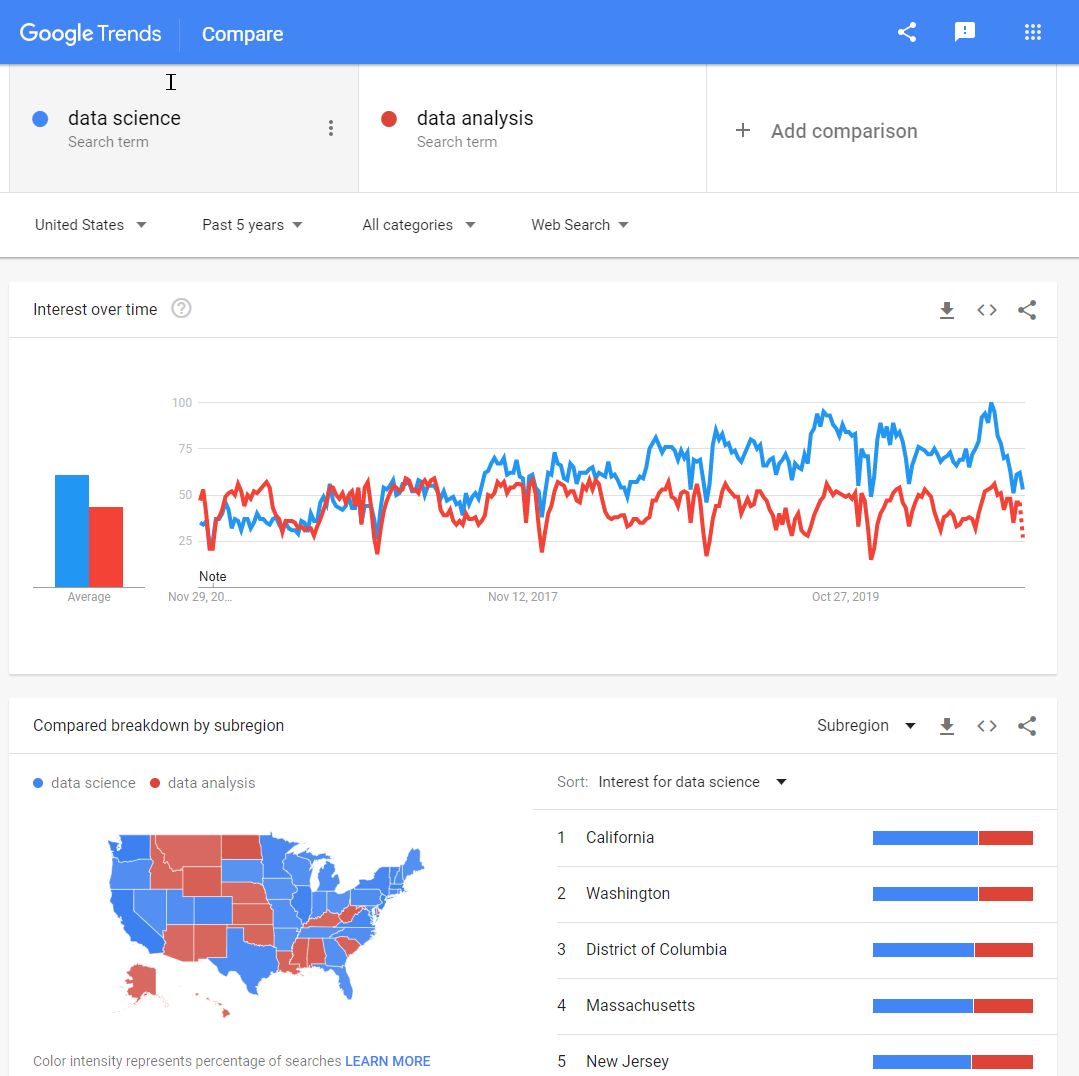
\includegraphics[trim = 0 0 0 0,clip,width=\textwidth]{figures/google.png} }
    \end{center}
        \hrule
        \vspace{2mm}
    \caption{ \textbf{Google Trends: Web-search Demand:} \newline \footnotesize { Web search is defined as a user going to Google and typing in a key word.  The time-series graph shows the demand for the past 5 years.  About mid-2017, \textbf{\tt{Data science}} became a hot-topic and search-demand has been trending upward since.  \textbf{\tt{Data analysis}}, on the other hand, seems to be a steady trend. \newline [Both trend lines appear to have a significant seasonal drop-off around the winter holidays.]  \newline \newline In our estimation, tied to this "hot-topic" label was a perception that there were a lot of \emph{cush jobs} out there that were high paying.  Second-tier educational platforms to increase their revenues likely feed this frenzy. \newline \newline \textbf{It is essential to emphasize that this is web-search demand, not \underline{Job Market Demand}.}  \newline [High-resolution, interactive visualization: \url{https://bit.ly/2V1pgc5}]   }  }
    \vspace{2mm}
    \hrule
\end{figure}

\newpage
\section{ Demand in Marketplace}
\label{sec:dm}

Since mid July 2020, we have been tracking the pulse of the job market
in the data domain. Some hiring companies choose one website over
another; some choose multiple websites. Although there are many
different job-posting websites, we identified \emph{Monster.com} and
\emph{Indeed.com} as two major players with a significant reach and
history. Of those two, \emph{Indeed.com} has the fewest barriers for a
small business to post a job, see (\url{https://bit.ly/2J937X1}). If a
hiring company never chooses to promote their job, the use of the
website costs nothing. \emph{Monster.com} charges a little under \$300
per job posting. Based on this simple economics hurdle, we chose
\emph{Indeed.com} for our initial analysis. Although not comprehensive,
this choice prevents possible overlap and does represent hiring
companies actively seeking workers.

Every week (midnight between Sunday/Monday), a scheduled script would
run that would harvest the first page of results for a given keyword
(e.g, \url{https://indeedhi.re/33f29za}). This page would be collected,
curated, and parsed to return the total number of jobs related to the
keyword.

\begin{figure}[!ht]
    \label{fig:indeed-search}
%% figures have hrule, tables have hline
    % \hrule
    \begin{center}
        \scalebox{1.00}{    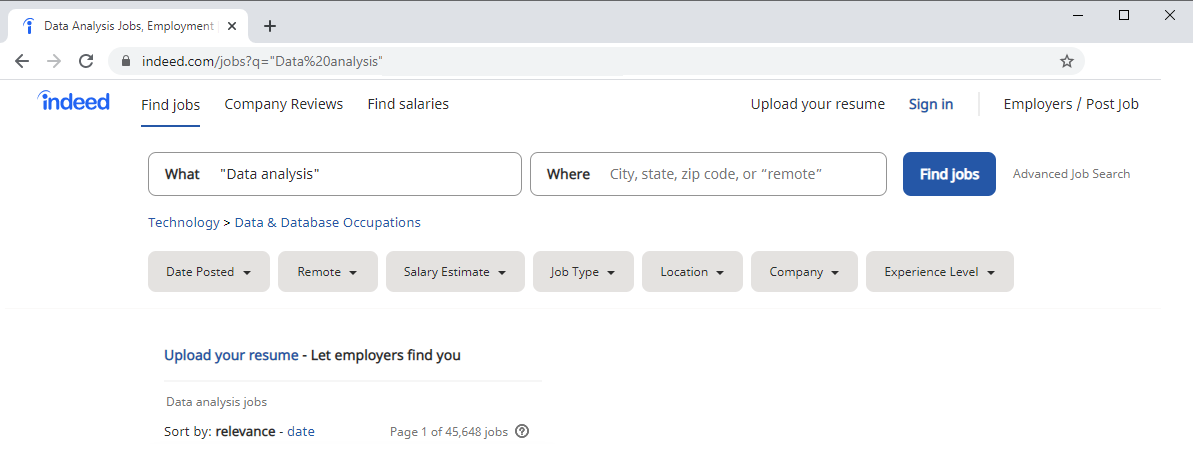
\includegraphics[trim = 0 0 0 0,clip,width=\textwidth]{figures/indeed.png} }
    \end{center}
        \hrule
        \vspace{2mm}
    \caption{ \textbf{\emph{Indeed.com} example search:} \newline \footnotesize { In this example, (November 25), we perform a search for the exact phrase \textbf{\tt{Data analysis}}; see \url{https://indeedhi.re/33f29za}  }  }
    \vspace{2mm}
    \hrule
\end{figure}

Figure \ref{sec:intro} provides a summary of this counting procedure for
a few months now. With the little data we have at the moment, trending
does not seem relevant so we report the average jobs counts for a
relevant keyword from July 14 to November 22, 2020. If you were to
perform an exact search comparing \textbf{\tt{Data analysis}}
(\url{https://indeedhi.re/33f29za}) to \textbf{\tt{Data science}}
(\url{https://indeedhi.re/2J9sWpJ}) today, you would see about a 2x
factor: there are twice as many active job postings with
\textbf{\tt{Data analysis}} (about 40,000) than
\textbf{\tt{Data science}} (about 20,000).

\newpage

\noindent This may be an indicator of the national economy: hiring is
happening but very judiciously and frugally. Hiring managers want a
strong value proposition for a new recruit. Two data analysts each
making between \$40,000 and \$65,000 is better than one data scientist
making about \$125,000.

There is a bit of conjecture in this current conclusion. It is based on
qualitative data: reading forums, manually reviewing a few job postings,
talking to students actively seeking employment and so on. As a
foundation, this qualitative assessment with the preliminary job-count
analysis does seem to indicate that a value proposition as put forth by
the WSU data-analytics department (\textbf{\tt{Data analysis}}) is
appropriate.

Future research would do more than just count the jobs. Each job
application would be download, curated, and relevant factors from the
job posting would be extracted: skill requirements, expected salary,
interaction of keywords, and other trends using natural-language
processing and social-network analyses. Such analysis will provide a
deeper understanding of the market, and plans are in place to begin the
harvesting of relevant job documents from Indeed.com in January 2021.
Such a unique data set will provide the program with ongoing insights to
maintain an understanding of demand as the market evolves. The initial
harvest will be over a million job documents and the weekly update would
be approximately 10,000 new jobs.

\section{Conclusion}
\label{sec:conclusion}

University resources are limited. As such, any program development
should have a justifiable value proposition. In this preliminary
research, we explore the potential demand in the marketplace for
students earning undergraduate and advanced degrees in Data Analytics.
Although our current data-collection approach has its limits, data
analytics appears to be something the market is demanding (more so than
data science).

Albeit exploratory, this preliminary conclusion may present a unique
opportunity for Washington State University. An emphasis on what the
market demands: ``data analysis'' over ``data science'' (which is
marketed by educational institutions as ``cool'' but may in fact be not
well received by the market: not enough emphasis on communication
(liasion), on fundamental analytical skills (statistican over
``black-box'' operator), and too theoretical (not solving real-world
problems grounded in business contexts).

In conclusion, we do see a value proposition for WSU if the program as
properly branded as data analytics. We can extend our understanding of
these initial insights by collecting more job-related data from this
same data source. We plan on beginning that data endeavor in January
2021.




%% appendices go here!


\newpage
\theendnotes

%%%%%%%%%%%%%%%%%%%%%%%%%%%%%%%%%%%  biblio %%%%%%%%
\newpage
\begin{auxmulticols}{1}
\singlespacing 
\bibliography{./../../latex-setup/biblio/master.bib}

%%%%%%%%%%%%%%%%%%%%%%%%%%%%%%%%%%%  biblio %%%%%%%%
\end{auxmulticols}

\newpage
{
\hypersetup{linkcolor=black}
\setcounter{tocdepth}{3}
\tableofcontents
}



\end{document}